%% All authors must submit their articles at
%% \href{http://www.pnascentral.org/cgi-bin/main.plex}{PNAScentral}. If
%% you are using Overleaf to write your article, you can use the ``Submit
%% to PNAS'' option in the top bar of the editor window.

\documentclass[9pt,twocolumn,twoside,lineno]{pnas-new}
% Use the lineno option to display guide line numbers if required.

\templatetype{pnasresearcharticle} % Choose template 
% {pnasresearcharticle} = Template for a two-column research article
% {pnasmathematics} %= Template for a one-column mathematics article
% {pnasinvited} %= Template for a PNAS invited submission

\title{Genotypic variation in a foundation tree directs ecological
  network structure}

% Use letters for affiliations, numbers to show equal authorship (if applicable) and to indicate the corresponding author
\author[a,b,1]{Matthew K. Lau}
\author[b]{Louis J. Lamit}
\author[c]{Rikke R. Naesbourg}
\author[d]{Stuart R. Borrett}
\author[e]{Matthew A. Bowker}
\author[a]{Thomas G. Whitham}

%% Include department, institution, and complete address, with the
%% ZIP/postal code, for each author. Use lower case letters to match
%% authors with institutions, as shown in the example. 
%% Authors with an ORCID ID may supply this information at submission.

\affil[a]{Department of Biological Sciences and Merriam-Powell Center
  for Environmental Research, Northern Arizona University, Flagstaff,
  AZ 86011, USA}
\affil[b]{Harvard Forest, Harvard University, 324 N Main St,
  Petersham, MA 01366, USA}
\affil[c]{University of California Berkeley, Berkeley, CA, USA}
\affil[d]{Department of Biology and Marine Biology, University of
  North Carolina Wilmington, 601 South College Road, Wilmington, NC, 28403, USA}
\affil[e]{School of Forestry, Northern Arizona University, Flagstaff, AZ 86011, USA}

% Please give the surname of the lead author for the running footer
\leadauthor{Lau} 
% Use letters for affiliations, numbers to show equal authorship (if applicable) and to indicate the corresponding author
% Please add here a significance statement to explain the relevance of your work
\significancestatement{Authors must submit a 120-word maximum
  statement about the significance of their research paper written at
  a level understandable to an undergraduate educated scientist
  outside their field of speciality. The primary goal of the
  Significance Statement is to explain the relevance of the work in
  broad context to a broad readership. The Significance Statement
  appears in the paper itself and is required for all research
  papers.}

% Please include corresponding author, author contribution and author declaration information

\authorcontributions{M.L. and L.L. conceived the study, M.L. and
  L.L. conducted the field work, R.N.  assisted in lichen
  identifications, M.L. wrote the first draft of the manuscript,
  S.B. and T.W. contributed substantively to the conceptual
  development, T.W. established the common garden. All authors
  contributed to revisions of the manuscript.}
\authordeclaration{The authors have no conflicts of interest.}
\correspondingauthor{\textsuperscript{1}Dr. Matthew K. Lau. E-mail: matthewklau@fas.harvard.edu}

% Keywords are not mandatory, but authors are strongly encouraged to
% provide them. If provided, please include two to five keywords,
% separated by the pipe symbol, e.g:
\keywords{Keyword 1 $|$ Keyword 2 $|$ Keyword 3 $|$ ...} 

\begin{abstract}
%% Please provide an abstract of no more than 250 words in a single
%% paragraph. Abstracts should explain to the general reader the major
%% contributions of the article. References in the abstract must be
%% cited in full within the abstract itself and cited in the text.

%% Currently: 272 words 13Dec2018

Biological evolution occurs in the context of complex networks of
interacting species in which natural selection defines the structure
of ecological networks. Fundamental to this evolutionary process is
the discovery of a genetic basis to ecological network
structure. Although previous work has demonstrated that tree genotype
contributes to interaction network structure at the scale of forest
stands, the contribution of tree genetics to localized interaction
networks at the scale of individual trees has not yet been
explored. To test the degree to which tree genetics can contribute to
network structure across scales from trees to stands, we conducted
quantitative modeling of interaction network for a community of
epiphytic lichens in a long-term experimental common garden of
genotyped trees of a foundation species (\textit{Populus
  angustifolia}). We found three main results: 1) Tree genotype
strongly contributed to network structure explaining over a third of
the variation in lichen interaction networks, 2) Multiple aspects of
interaction network structure varied in response to genotype,
including network size, the number of interactions, linkage density
and connectance, 3) At the stand scale, we also found signficant
modular structure of plant-lichen networks resulting in part from the
combination of trees of the same genotype tending to have similar
community compositions and supporting similar lichen interaction
networks dominated by positive interactions. These results support the
hypothesis that variation in ecological interaction networks can
result from genetically based variation in foundation
species. Although these results are for a community of sessile
organisms in close proximity to the tree, this study opens the
possibility for a genetic basis to both direct and indirect
interactions among species in complex communities.

\end{abstract}

\dates{This manuscript was compiled on \today}
\doi{\url{www.pnas.org/cgi/doi/10.1073/pnas.XXXXXXXXXX}}

\begin{document}

%% Many authors find it useful to organize their manuscripts with the
%% following order of sections; Title, Author Affiliation, Keywords,
%% Abstract, Significance Statement, Results, Discussion, Materials
%% and methods, Acknowledgments, and References. Other orders and
%% headings are permitted.

%% PNAS generally uses a two-column format averaging 67 characters,
%% including spaces, per line. The maximum length of a Direct
%% Submission research article is six pages and a Direct Submission
%% Plus research article is ten pages including all text, spaces, and
%% the number of characters displaced by figures, tables, and
%% equations.  When submitting tables, figures, and/or equations in
%% addition to text, keep the text for your manuscript under 39,000
%% characters (including spaces) for Direct Submissions and 72,000
%% characters (including spaces) for Direct Submission Plus.

%% Authors may use 1- or 2-column equations in their article,
%% according to their preference.

%% To allow an equation to span both columns, use the
%% \verb|\begin{figure*}...\end{figure*}| environment mentioned above
%% for figures.

%% Note that the use of the \verb|widetext| environment for equations
%% is not recommended, and should not be used.

%% \begin{figure*}[bt!]
%% \begin{align*}
%% (x+y)^3&=(x+y)(x+y)^2\\
%%        &=(x+y)(x^2+2xy+y^2) \numberthis \label{eqn:example} \\
%%        &=x^3+3x^2y+3xy^3+x^3. 
%% \end{align*}
%% \end{figure*}


%% \begin{table}%[tbhp]
%% \centering
%% \caption{Comparison of the fitted potential energy surfaces and ab initio benchmark electronic energy calculations}
%% \begin{tabular}{lrrr}
%% Species & CBS & CV & G3 \\
%% \midrule
%% 1. Acetaldehyde & 0.0 & 0.0 & 0.0 \\
%% 2. Vinyl alcohol & 9.1 & 9.6 & 13.5 \\
%% 3. Hydroxyethylidene & 50.8 & 51.2 & 54.0\\
%% \bottomrule
%% \end{tabular}

%% \addtabletext{nomenclature for the TSs refers to the numbered species in the table.}
%% \end{table}

%% References should be cited in numerical order as they appear in
%% text; this will be done automatically via bibtex,
%% e.g. \cite{belkin2002using} and
%% \cite{berard1994embedding,coifman2005geometric}. All references
%% should be included in the main manuscript file.

%% PNAS must be able to archive the data essential to a published
%% article. Where such archiving is not possible, deposition of data
%% in public databases, such as GenBank, ArrayExpress, Protein Data
%% Bank, Unidata, and others outlined in the Information for Authors,
%% is acceptable.


%% Only TIFF, EPS, and high-resolution PDF for Mac or PC are allowed
%% for figures that will appear in the main text, and images must be
%% final size. Authors may submit U3D or PRC files for 3D images;
%% these must be accompanied by 2D representations in TIFF, EPS, or
%% high-resolution PDF format.  Color images must be in RGB (red,
%% green, blue) mode. Include the font files for any text.

%% Figures and Tables should be labelled and referenced in the
%% standard way using the \verb|\label{}| and \verb|\ref{}| commands.

%% Figure \ref{fig:frog} shows an example of how to insert a
%% column-wide figure. To insert a figure wider than one column,
%% please use the \verb|\begin{figure*}...\end{figure*}|
%% environment. Figures wider than one column should be sized to 11.4
%% cm or 17.8 cm wide. Use \verb|\begin{SCfigure*}...\end{SCfigure*}|
%% for a wide figure with side captions.

%% Authors should submit SI as a single separate PDF file, combining
%% all text, figures, tables, movie legends, and SI references.  PNAS
%% will publish SI uncomposed, as the authors have provided it.
%% Additional details can be found here:
%% \href{http://www.pnas.org/page/authors/journal-policies}{policy on
%% SI}.  For SI formatting instructions click
%% \href{https://www.pnascentral.org/cgi-bin/main.plex?form_type=display_auth_si_instructions}{here}.
%% The PNAS Overleaf SI template can be found
%% \href{https://www.overleaf.com/latex/templates/pnas-template-for-supplementary-information/wqfsfqwyjtsd}{here}.
%% Refer to the SI Appendix in the manuscript at an appropriate point
%% in the text. Number supporting figures and tables starting with S1,
%% S2, etc.

%% Authors who place detailed materials and methods in an SI Appendix
%% must provide sufficient detail in the main text methods to enable a
%% reader to follow the logic of the procedures and results and also
%% must reference the SI methods. If a paper is fundamentally a study
%% of a new method or technique, then the methods must be described
%% completely in the main text.


\maketitle
\thispagestyle{firststyle}
\ifthenelse{\boolean{shortarticle}}{\ifthenelse{\boolean{singlecolumn}}{\abscontentformatted}{\abscontent}}{}

% If your first paragraph (i.e. with the \dropcap) contains a list
% environment (quote, quotation, theorem, definition, enumerate,
% itemize...), the line after the list may have some extra
% indentation. If this is the case, add \parshape=0 to the end of the
% list environment.

%% \dropcap{T}his PNAS journal template is provided to help you write
%% your work in the correct journal format.  Instructions for use are
%% provided below.

%% Note: please start your introduction without including the word
%% ``Introduction'' as a section heading (except for math articles in
%% the Physical Sciences section); this heading is implied in the
%% first paragraphs.

\dropcap{E}volution occurs in the context of complex networks of
interacting species. In ecological communities, community dynamics
depend on key interactions \cite{Fontaine2011} that occur in species
interaction networks, such as:  trophic \cite{Bascompte2006} and
mutualistic \cite{Rafferty2013} interaction networks. Phylogenetic
patterns in ecological networks support the importance of evolutionary
processes in shaping species interactions, community structure and
ecosystem processes \cite{Crutsinger 2016, Rezende2007,
  Whitham2006a}. Community genetics studies \cite{Lamit et al. 2015}
have shown that genetic variation in foundation species
\cite{Ellison2005} plays a significant role in defining distinct
communities of interacting organisms:  such as, endophytes, pathogens,
lichens, arthropods, and soil microbes. Multiple studies have now
demonstrated that genetic variation influences numerous functional
traits (e.g., phytochemical, phenological, morphological) produces a
multivariate phenotype \cite{holeski2012} tha contributes to variation
in associated communities \cite{Bailey2009a}.


Additional work has provided support for the hypothesis that not only
does composition vary among genetically distinct genotypes of
foundation species but it also impacts the structure of the network of
species interactions in these communities \cite{Keith2017,
  Lau2016}. Also, work by \citep{Toju 2018, Toju2015, Toju2014}
observed consistent patterns of centralized interactions of species
modules focused around hubs of plant-fungal interactions. In other
words, a small number of plant and fungal symbionts tended to have
have disproportionate numbers of interactions with other species and
likely are the drivers in determining community assembly, structure
and dynamics.

Here, we investigate how genetic variation in a foundation tree
species determines the structure of a network of interactions among a
community of lichen species. Using a long-term (20 years+), common
garden experiment with replicated individuals of known genetic
identity and a naturally established stand of
\textit{P. angustifolia}. We focused on a model community of 9
epiphytic lichens species, as previous research has demonstrated
significant compositional responses of epiphytes to genotypic
variation \cite{Winfree2011, Zytynska2011}. In addition, the
life-history characteristics of lichen, having highly localized,
direct contact interactions and slow population turnover rates,
allowed us to assess interactions among lichen species on individual
trees. We hypothesize that in natural systems evolution occurs in a
community context involving interactions of complex networks of
interacting species \cite{Lau2016, Keith2017, Thompson2013,
  Bascompte2007, Darwin1855}.  If correct, we should expect to find
that network structure is genetically based in which different plant
genotypes support different interaction networks and that these
interactions networks can function as indicators of ecological
dynamics important for conserving biodiversity.  Applying a dual-scale
(lichen-lichen and genotype-lichen interactions) network modeling and
analyses, we then examined the genetically based impacts of
\textit{P. angustifolia} on network structure.


\matmethods{

\begin{itemize}
\item Common garden
  \begin{itemize}
  \item Cottonwoods in the west
  \item Restoration site
  \item Wild stand
  \end{itemize}
\item Lichen observations
  \begin{itemize}
  \item Grid system
  \item Two grids (upper and lower)
  \item Lichen size distribution (dominant Xgal)
  \end{itemize}
\item Network modeling
  \begin{itemize}
  \item Network modeling
  \item Elaborate from figure legend
  \end{itemize}
\item Network metrics
  \begin{itemize}
  \item Elaborate calculations and meanings
  \end{itemize}
\item Statistical analyses and software
  \begin{itemize}
  \item REML
  \item Least squares models
  \item PerMANOVA
  \item Mantel tests
  \item Code and data available via github and zenodo
  \end{itemize}
\end{itemize}


\subsection*{Field observations in common garden and natural riparian forest stands}

The study was conducted along the Weber River, UT (USA), which is a
cottonwood (\textit{Populus} spp.) dominated riparian
ecosystem. Although two native species, \textit{Populus angustifolia}
(James) and \textit{Populus fremontii} (S. Watson), occur here and are
known to hybridize, only pure or advanced generation backcrosses of
\textit{P. angustifolia} were sampled in order to avoid the effect of
the hybridization between these two species.

A common garden was used to isolate the effect of tree genotype from
the effect of the localized microenvironment associated with each
individual and spatial autocorrelation. Asexually propagated clones of
genotyped \textit{P. angustifolia} individuals were obtained from wild
collections and planted randomly in a single field (0.025 km$^2$) at
the Ogden Nature Center, Ogden, UT in 1992. A total of thirteen
genotypes replicated between 3 and 8 times each, were chosen for
sampling. Genotype names were previously published
\cite{Martinsen}. 

Observations were made in the common garden in October 2010 and May
2011. 

%% \begin{figure}%[tbhp]
%% \centering
%% \includegraphics[width=.8\linewidth]{frog}
%% \caption{Placeholder image of a frog with a long example caption to show justification setting.}
%% \label{fig:frog}
%% \end{figure}


%% \begin{SCfigure*}[\sidecaptionrelwidth][t]
%% \centering
%% \includegraphics[width=11.4cm,height=11.4cm]{frog}
%% \caption{This caption would be placed at the side of the figure, rather than below it.}\label{fig:side}
%% \end{SCfigure*}


\begin{figure}[ht]
\centering
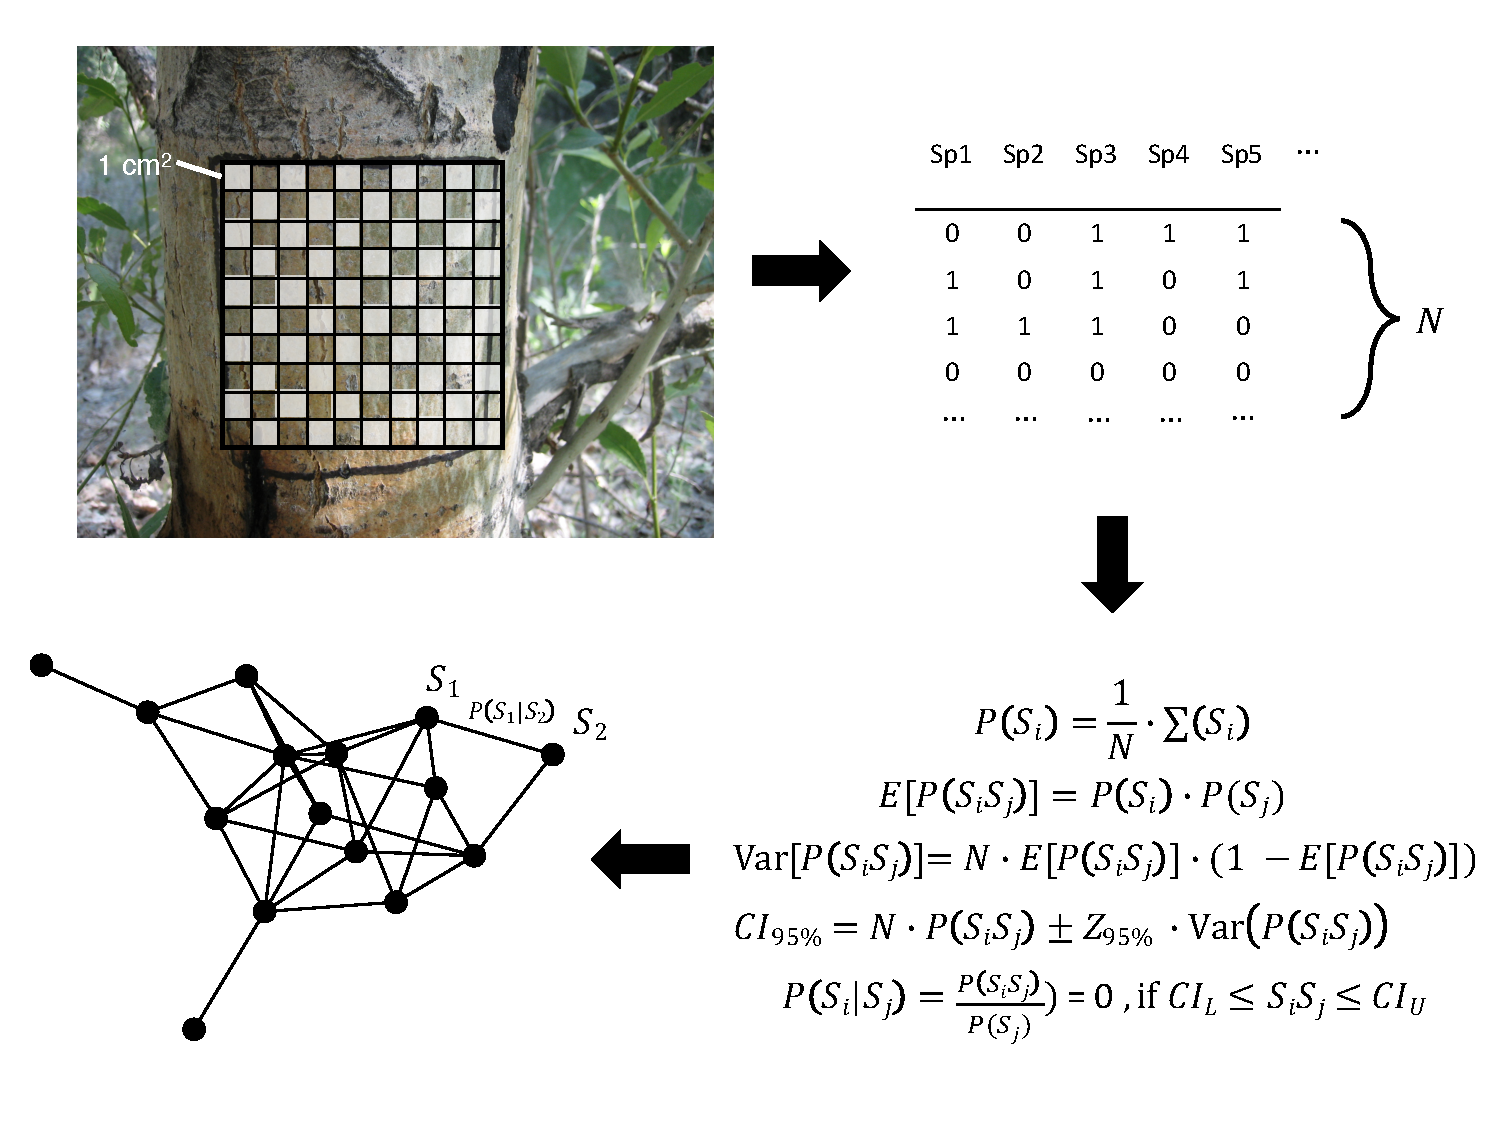
\includegraphics[width=\linewidth]{conet_method.pdf}
\caption{Lichen interaction networks were constructed by conducting
  field observations in 1 cm$^2$ cells within a 10 cm$^2$ grid on each
  tree using a checkerboard pattern (grey cells). Thus, a set of $N$
  total cell observations were recorded for each tree with the
  presence or absence of each species recorded for each cell. Applying
  a null-model based procedure \cite{Araujo2011}, we calculated and
  removed non-significant ($\alpha = 0.05$) co-occurrences to produce
  the network associated with an individual tree.}
\label{fig:conet_method}
\end{figure}


\textbf{Make a figure of the field site and lichen on trees}



\section*{Results}


%%% This subsection analyzes the respones of the
%%% bark lichen community to tree genotype 

Figure: Roughness response + community response

\subsection*{Bark characteristis and lichen respond to tree genotype}

\begin{itemize}
\item Genotype affected roughness (REML RLRT = 10.69, p-value = 3e-04)
\item Genotype affected total cover (REML RLRT = 2.9627, p-value = 0.0375)
\item Genotype didn't affect richness (REML RLRT = 0.13047, p-value = 0.3134)
\item Genotype predicted community composition (PerMANOVA R2 = 0.243,
  F 12 = 1.8221, p-value = 0.0029)
\item After controlling for genotype, cover (PerMANOVA R2 = 0.236, F 1
  = 21.2661, p-value = 9.999e-05) and richness (PerMANOVA spr.onc R2 =
  0.054, F 1 = 4.9036, p-value = 0.0011) predicted composition.
\item Roughness was correlated with total cover (LM F 1, 55 = 6.797,
  p-value = 0.01173)
\item Roughness was not correlated with richness (LM F 1, 55 = 1.509,
  p-value = 0.2246)
\item Roughness did not predict community composition, after
  controlling for genotype (PerMANOVA R2 = 0.011, F 1 = 0.9938,
  p-value = 0.3841)
\end{itemize}


%%% This subsection connects the community responses to
%%% network variation in response to tree genotype.

Figure: Genotype networks + Genotype network similarity by genotype

\subsection*{Tree genotype influenced lichen network similarity}

\begin{itemize}
\item Network structure across tree genotypes 
\item Lichen species varied in their centrality with
  \textit{C. subdeflexa} having the highest average centrality Cs
  0.92555555, Ch 0.61630902, Ls 0.47898268, Xg 0.22570664 Rs
  0.21010254 Pm 0.09072022 Xm 0.06850459 Pu 0.02192982, Pa 0.00000000
\item Genotype predicted network similarity (PerMANOVA R2 = 0.33795, F
  12 = 2.5379, p-value = 0.0050)
\item Species richness predicted network similarity after controlling
  for genotype (PerMANOVA R2 = 0.3413, F 1 = 2.5417, p-value =
  0.007399)
\item Neither total cover (PerMANOVA R2 = 0.023, F 1 = 2.0628, p-value
  = 0.1487) nor roughness (PerMANOVA R2 = 0.011, F 1 = 0.0497, p-value
  = 0.3394) predicted network similiarity
  \item Community similiarty was not correlated with network
  similiarity (Mantel Rho spearman = 0.012, p-value = 0.337)
\end{itemize}

%%% This subsection focuses on network metrics to illucidate the
%%% structural changes of networks.

Figure: Linkage and centrality by genotype
Figure: Total cover and species richness predict L and Cen

\subsection*{Lichen network patterns were primarily driven by linkages}

\begin{itemize}
\item Genotype marginally predicted linkage (REML RLRT = 2.0221,
  p-value = 0.0657) and centrality (REML RLRT = 2.0915, p-value =
  0.0627)
\item Genotype did not predict modularity (REML RLRT = 0.18429,
  p-value = 0.2941)
\item Total cover predicted links (ANOVA F 1 = 6.867, p-value = 0.0114)
  and centrality (ANOVA F 1 = 8.093, p-value = 0.0063) but not
  modularity (ANOVA F 1 = 2.2250, p-value = 0.1417).
\item Species richness predicted links (ANOVA F 1 = 29.436, p-value =
  1.46e-06), centrality (ANOVA F 1 = 39.488, p-value = 6.38e-08) and
  modularity (ANOVA F 1 = 31.2713, p-value = 8.004e-07).
\item Bark roughness did not predict the number of links (ANOVA F 1 =
  2.897, p-value = 0.0946), centrality (ANOVA F 1 = 2.591, p-value =
  0.1134) or modularity of the lichen networks (ANOVA F 1 = 0.511,
  p-value = 0.478).
\item The number of network links (PerMANOVA R2 = 0.392, F 1 =
  72.4348, p-value = 0.001) and network centrality (PerMANOVA R2 =
  0.309, F 1 = 57.0440, p-value = 0.001) were correlated with network
  similarity, but not modularity (PerMANOVA R2 = 0.013, F 1 = 2.4048,
  p-value = 0.105).
\end{itemize}

\subsection*{Heritability estimates for lichen networks}

Table: heritability

\begin{itemize}
\item Compare all trait heritabilities
\item 
\end{itemize}

% latex table generated in R 3.5.1 by xtable 1.8-3 package
% Thu Jan 17 20:13:56 2019
\begin{table}[ht]
\centering
\begin{tabular}{llll}
  \hline
Response & H2 & R2 & p-value \\ 
  \hline
  Percent Rough Bark           & 0.37835 & 0.37835 & 4e-04 \\ 
  Lichen Network               & 0.2784  & 0.3413  & 0.0074 \\ 
  Percent Lichen Cover         & 0.17279 & 0.17279 & 0.0362 \\ 
  Number of Network Links      & 0.16892 & 0.16892 & 0.0689 \\ 
  Network Centrality           & 0.17248 & 0.17248 & 0.0627 \\ 
  Lichen Community Composition & 0.08526 & 0.27703 & 0.09529 \\ 
  Network Modularity           & 0.04511 & 0.04511 & 0.2941 \\ 
  Lichen Species Richness      & 0.03578 & 0.03578 & 0.3137 \\ 
   \hline
\end{tabular}
\caption{Genotypic effects of cottonwood trees on the associated lichen community.} 
\label{tab:h2_table}
\end{table}

Supplementary: Stats tables


%% Not sure if these results should be included, it might be enough to
%% just tell the unipartite network story.
%% \subsection*{Genotypic variation increases stand-level lichen network modularity}
%% \begin{itemize}
%% \item Lichens displayed signficant bipartite network structure
%% \item Bipratite network structure was greater than compared to the
%%   modularity based on a null model that randomizes with respect to genotype
%% \item z = 856.05271, p-value <= 0.00100 
%% \end{itemize}

\begin{figure}[ht]
\centering
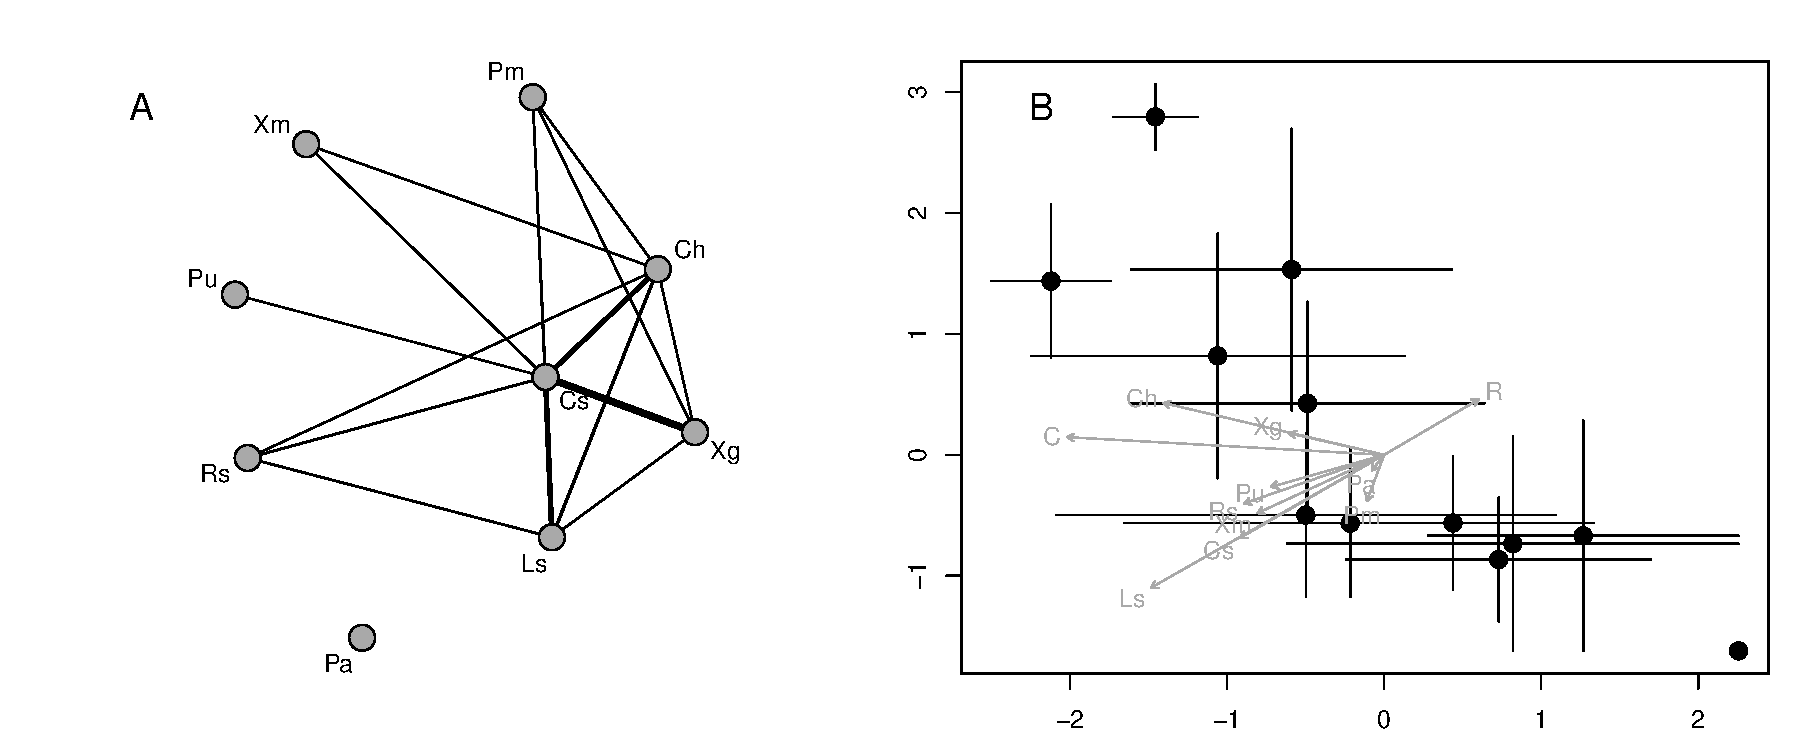
\includegraphics[width=\linewidth]{cn_chplot_onc.pdf}
\caption{Significant lichen interaction network structure resulting
  from tree genotypic variation was observed in the common garden. A)
  A network diagram showing significant interactions averaged over all
  trees shown as edges connecting lichen species shown as vertices. B)
  Genotype centroids (points) of NMDS ordinated lichen networks ($\pm$
  1 S.E.). Arrows show the magnitude and direction of correlation of
  the ordinated networks with tree bark roughness (R), network
  connectance and lichen species abundances (Xg =
  \textit{Xanthomendoza galericulata}, Xm = \textit{X. montana}, Ch =
  \textit{Caloplaca holocarpa}, Cs = \textit{Candelariella
    subdeflexa}, Rs = \textit{Rinodina} (unknown species), Ls =
  \textit{Lecanora} (unknown species), Pm = \textit{Phyciella
    melanchra}, Pa = \textit{Physcia adscendens}, Pu = \textit{Physcia
    undulata}).}
\label{fig:ch_plot}
\end{figure}

%% In addition to including your tables within this manuscript file, PNAS
%% requires that each table be uploaded to the submission separately as a
%% “Table” file.  Please ensure that each table .tex file contains a
%% preamble, the \verb|\begin{document}| command, and the
%% \verb|\end{document}| command. This is necessary so that the
%% submission system can convert each file to PDF.


% latex table generated in R 3.4.4 by xtable 1.8-2 package
% Tue Nov 13 15:56:44 2018
\begin{table}[ht]
\centering
\begin{tabular}{llll}
  \hline
Response & Predictor & p-value & H2 \\ 
  \hline
Percent Lichen Cover & Tree Genotype & 0.0356 & 0.17 \\ 
  Lichen Species Richness & Tree Genotype & 0.1443 & 0.1 \\ 
  Percent Rough Bark & Tree Genotype & 8e-04 & 0.38 \\ 
  Lichen Network & Genotype & 0.0431 & 0.17 \\ 
  Number of Network Links & Genotype & 0.0796 & 0.15 \\ 
  Network Centrality & Genotype & 0.1351 & 0.12 \\ 
   &  &  &  \\ 
   &  &  &  \\ 
   &  &  &  \\ 
   \hline
\end{tabular}
\caption{Genotypic effects of cottonwood trees on the associated lichen community.} 
\label{tab:h2_table}
\end{table}


%% \begin{figure}[ht]
%% \centering
%% \includegraphics[width=\linewidth]{}
%% \caption{}
%% \label{fig:}
%% \end{figure}

\begin{figure}[ht]
\centering
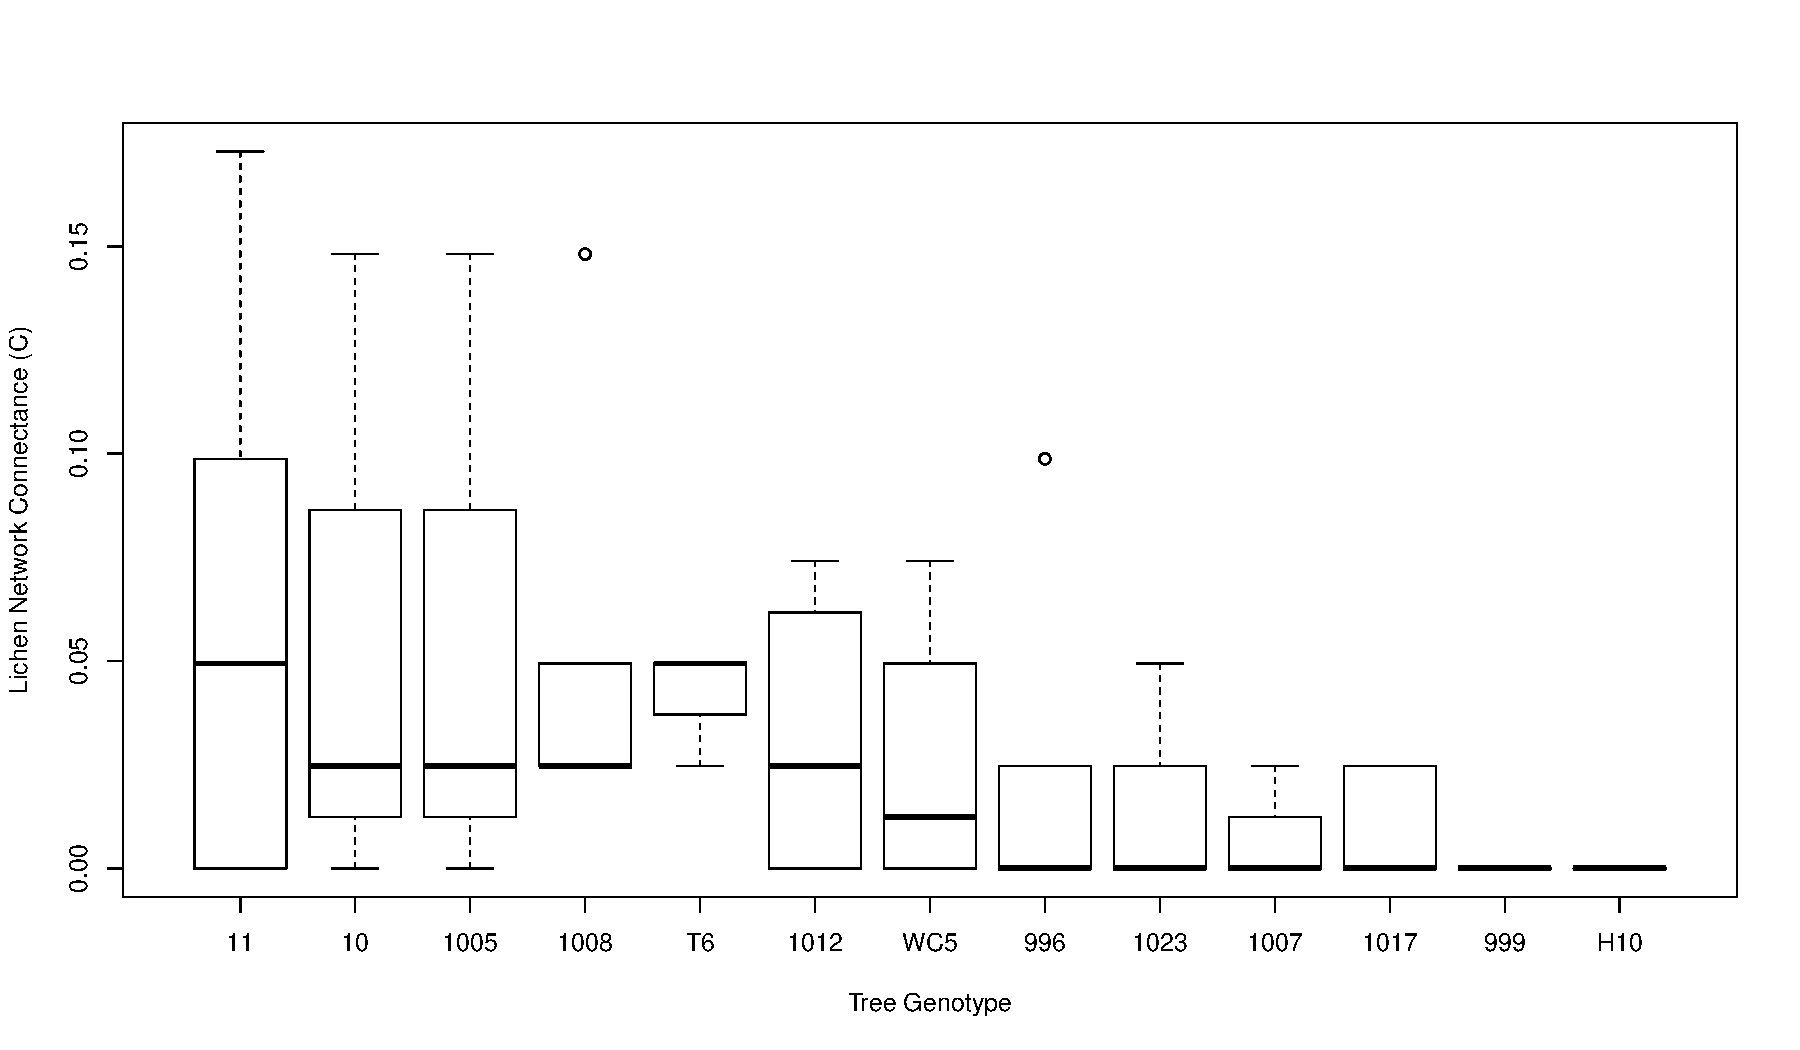
\includegraphics[width=\linewidth]{connect_geno.pdf}
\caption{Connectance significantly varied among genotypes.}
\label{fig:connect}
\end{figure}


\begin{figure}
\centering
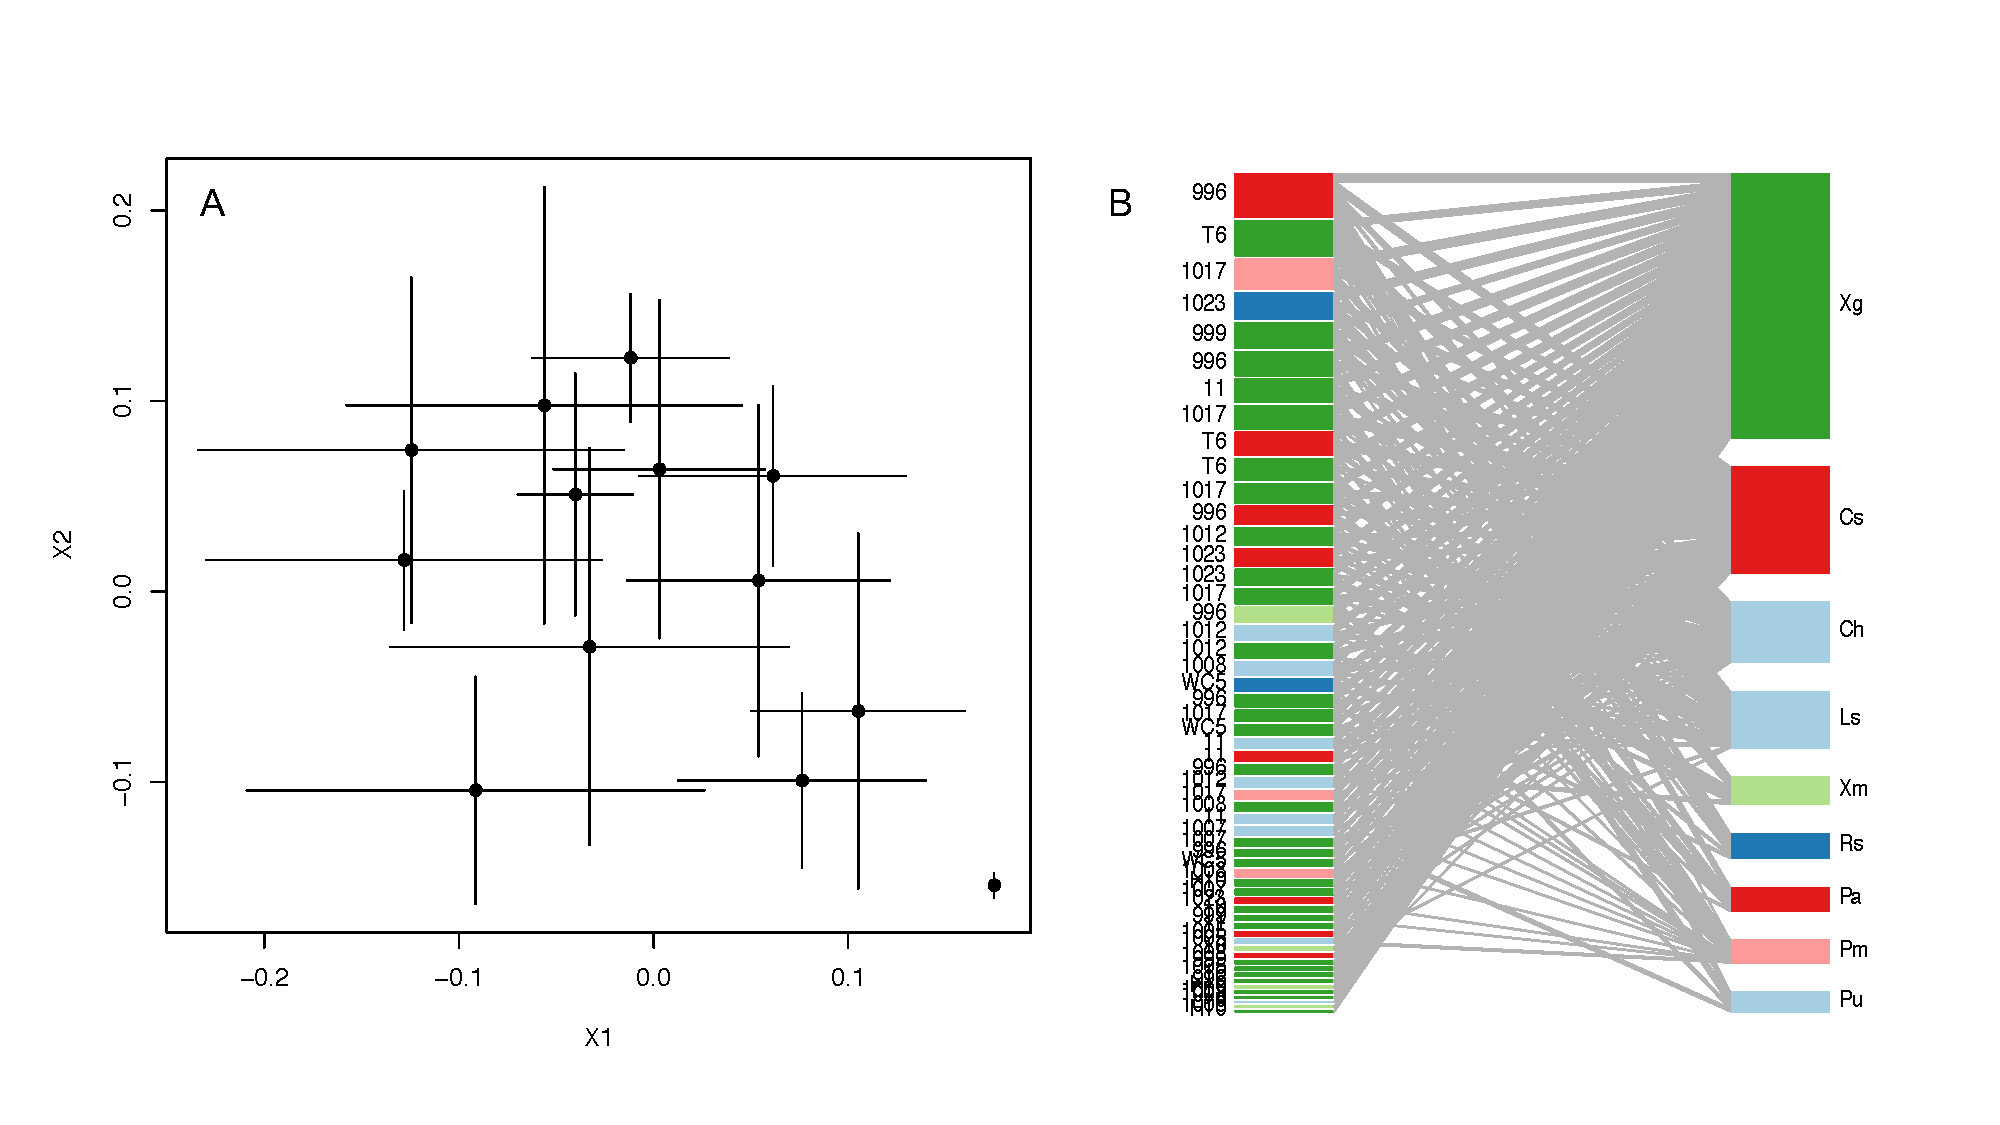
\includegraphics[width = \textwidth]{lcn_com_bpnet.pdf}
%% 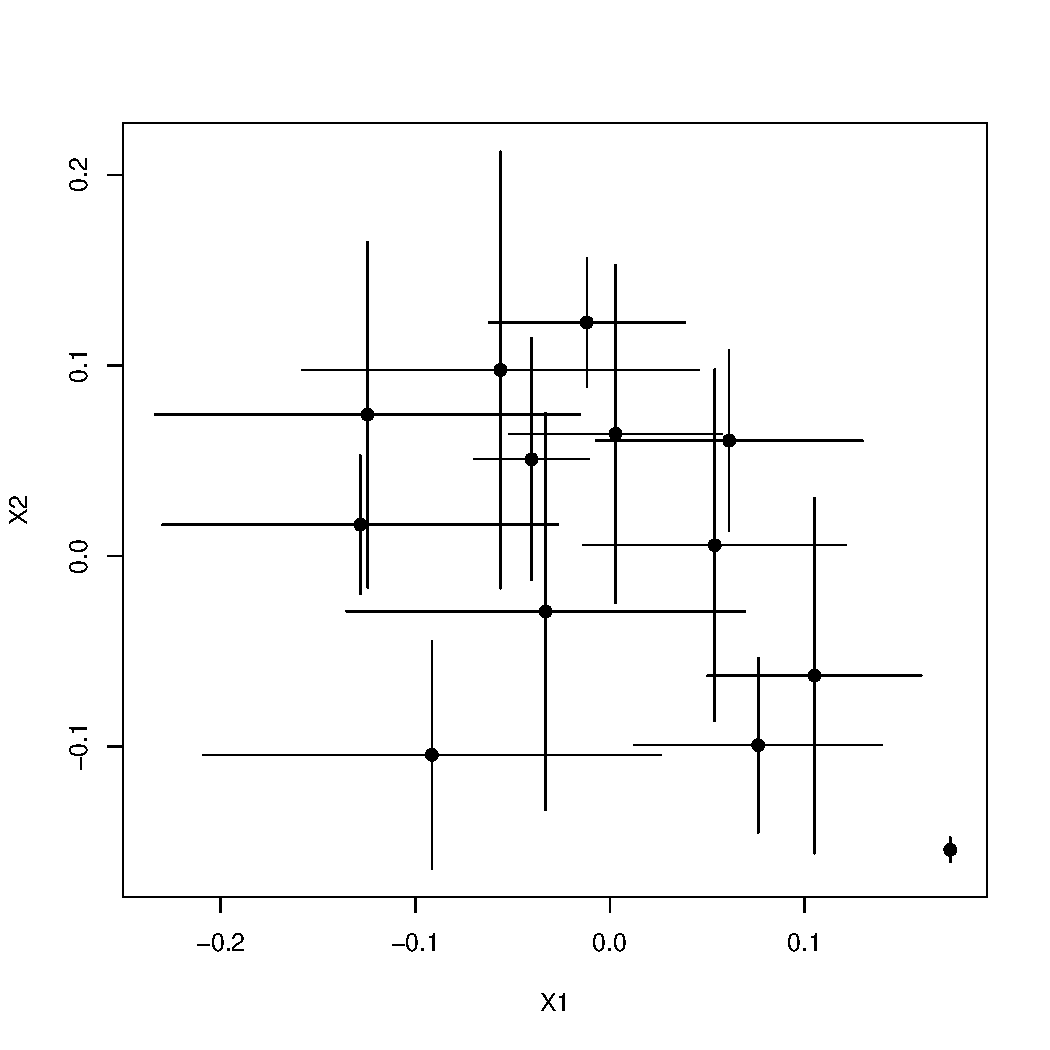
\includegraphics[width = 0.4\textwidth]{chp_com_onc.pdf}
%% 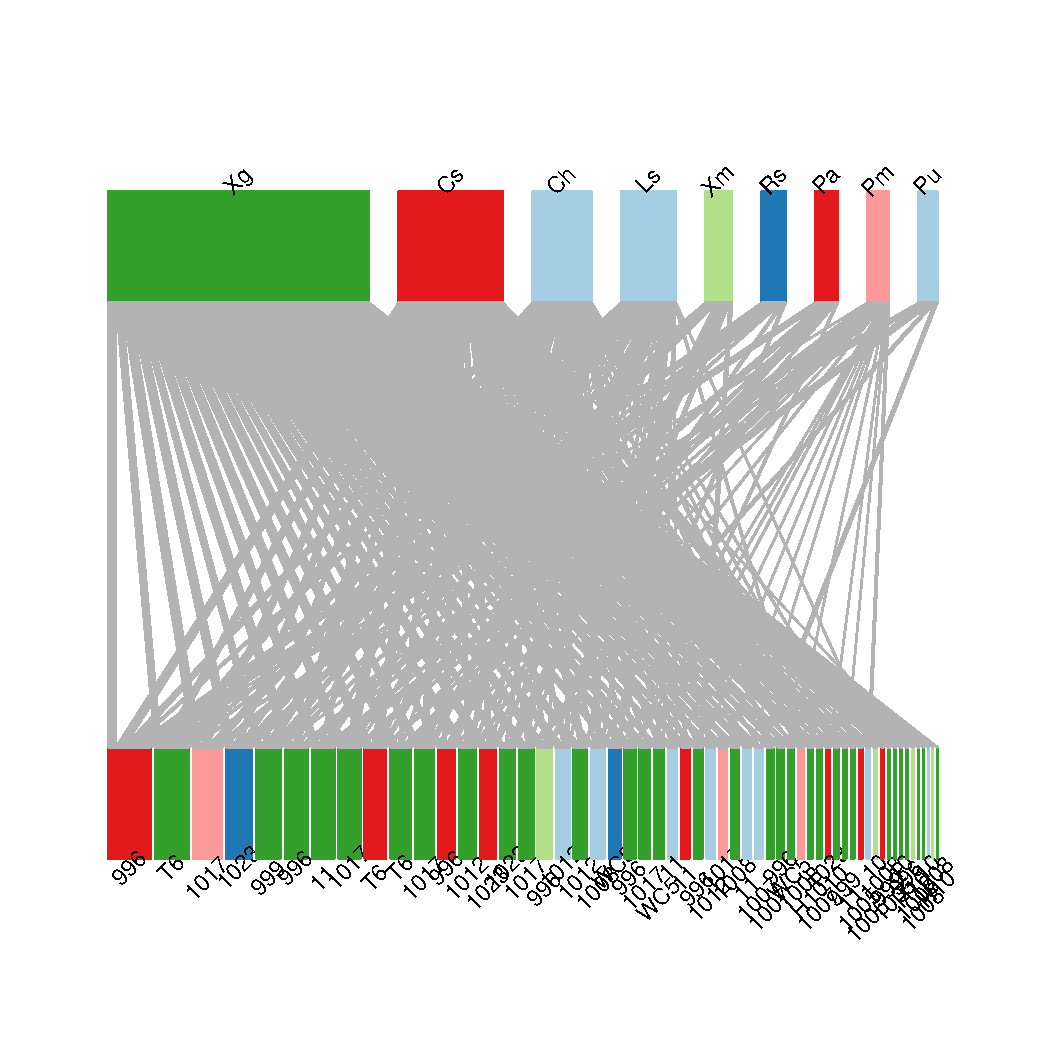
\includegraphics[width = 0.4\textwidth, angle = -90]{bp_net_onc.pdf}
\caption{Tree genotype varition in lichen community composition also
  contributed to genotype-species bipartite intreraction network
  structure at the scale of the common garden stand. A) Plot of the
  ordinated community composition scores shown as centroids ($\pm$ 1
  S.E.). B) Bipartite interaction network based on the occurrences of
  lichen on individual cottonwood trees in the common garden. Edges
  connecting trees to lichen are scaled by the relative abundance of
  lichen. Nodes of lichen and trees are colored by their module
  membership.}
\label{fig:bpnet}
\end{figure}




}


\showmatmethods{} % Display the Materials and Methods section


\section*{Discussion}

\begin{itemize}
\item Rehash of results support hypothesis of genetic basis to network structure
\item Genotypic environmental filtering leads to altered interaction
  network structure and potentially dymanics
\item Indirect effects of genotypes (G -> rough -> cover -> richness
  -> links -> networks)
\item Importance of indirect effects and complexity and releveance to IIGEs
\item Conclusion
\end{itemize}



Trait variation + assembly + ecosystem function

These findings support the hypothesis that genotypic variation in a
foundation species contributes to the structure of a network of
interacting species that might be least expected to exhibit such
structure. 

\textbf{TGW: MIGHT BE GOOD TO CITE PAPERS ON COMEPTITION IN LICHENS OR
OTHER ORGANIZING FACTORS TO BACK UP THE LEAST EXPECTED STATEMENT.  AS
EPIPHYTES WE MIGHT NOT EXPECT THEM TO CARE.}

\textbf{MKL: This is a job for Lamit and Rikke.}

Several lines of evidence support this conclusion. First, the wild
stand showed significant interaction network structure (Fig. 1a and
b); and both tree genotype and the genetically based tree trait, bark
roughness, was a strong predictor of co-occurrence patterns
(Fig. 2a). 

\textbf{TGW: I THINK WE NEED TO EMPHASIZE THE LONG-TERM NATURE OF OUR
COMMON GARDEN STUDY AS VERY FEW COMMON GARDEN STUDIES OF LICHENS
LIKELY EXIST. ANY REFS ON THIS? IF TRUE MIGHT WANT TO MENTION THIS UP
FRONT IN INTRO.}

\textbf{MKL: Same here. This is a job for Lamit and Rikke.}

Second, in a long-term common garden study, network
(Fig. 1b) structure showed a high degree of similarity to the wild
stand network structure (Fig. 1c and d). Third, tree genotype was a
significant predictor of SES values (Fig. 2a), displaying significant
correlation with a genetically linked trait, bark roughness, both in
the common garden (Fig. 2a) and in a naturally established stand of
trees (Fig. 2b). Last, both of the bipartite genotype-species networks
in the common garden and natural stand displayed significant
modularity, suggesting that genotypic variation is leading to the
formation of evolutionarily dynamic compartments within the
community. Thus, just as numerous studies have shown that plant
genotype can affect species richness, abundance, diversity, and
composition and previous work has demonstrated that evolutionary
processes shape ecological networks \cite{Guimaraes2011,
  Moya-Larano2011}, our study includes genetics in an empirical
investigation that combines both experimental common garden findings
along with studies in the wild that are in close agreement.

Our results point to the importance of understanding the community
level effects of genetic variation and corroborate previous findings
of the importance of plant genetics in shaping community structure and
ecosystem processes \cite{Whitham2006a}.  This study highlights the
potential for indirect effects of genetic variation to propagate
through networks of interacting species and trophic levels. Altering
the structure of interaction networks presents a means for genetic
effects to be magnified within the system of interacting species. For
example, Keith et al. (2017) showed that the genetics based
interations of aphid resistant and aphid susceptible trees resulted in
different interaction networks of their associated arthropod
communities composed of 139 species. At the scale of ecosystems,
trophic networks or food webs direct and control the rates of energy
and nutrient flux \cite{Borgatti2006}. Furthermore, in a
predator-prey-plant study, Smith \cite{Smith2011}, showed that the
interactions among species across trophic levels depended on plant
genotype.

\subsection{Units of evolutionary potential: Moving beyond species pairs}


Although our study was conducted with a community of lichens, these
results should be generalized to other groups of diverse organisms
around the world that also exhibit significant genetic signals at the
community level \cite{Rowntree2011, Whitham2012}, although spatial
scale of interactions should be considered \cite{Zook2010} Bangert et
al. 2006. As heritable variation is the raw material for natural
selection to act upon, a genetic basis for interaction network
structure indicates evolutionary dynamics should be considered at the
community level and that conserving genetic variation is important to
consider in efforts to restore or preserve complex species
interactions and their associated ecosystem functions
\cite{Evans2013}.  With such findings, it appears that we are closer
to understanding the evolutionary drivers of Darwin's entangled bank
and the interconnectedness of species in complex communities.

%% Please include your acknowledgments here, set in a single
%% paragraph. Please do not include any acknowledgments in the
%% Supporting Information, or anywhere else in the manuscript.

\acknow{This work was supported by the National Science Foundation grant
(DEB-0425908) and Integrative Graduate Research Traineeship (IGERT)
fellowships for M.L. and L.L. The Ogden Nature Center staff helped to
maintain the common gardens. Lichen sampling was supported by Todd
Wojtowicz, Luke Evans and David Solance Smith.}

\showacknow{} % Display the acknowledgments section

\bibliography{lichen_network_genetics}

\end{document}

%% \subsection*{Supporting Information (SI)}

%% Authors should submit SI as a single separate PDF file, combining
%% all text, figures, tables, movie legends, and SI references.  PNAS
%% will publish SI uncomposed, as the authors have provided it.
%% Additional details can be found here:
%% \href{http://www.pnas.org/page/authors/journal-policies}{policy on
%% SI}.  For SI formatting instructions click
%% \href{https://www.pnascentral.org/cgi-bin/main.plex?form_type=display_auth_si_instructions}{here}.
%% The PNAS Overleaf SI template can be found
%% \href{https://www.overleaf.com/latex/templates/pnas-template-for-supplementary-information/wqfsfqwyjtsd}{here}.
%% Refer to the SI Appendix in the manuscript at an appropriate point
%% in the text. Number supporting figures and tables starting with S1,
%% S2, etc.

%% Authors who place detailed materials and methods in an SI Appendix
%% must provide sufficient detail in the main text methods to enable a
%% reader to follow the logic of the procedures and results and also
%% must reference the SI methods. If a paper is fundamentally a study
%% of a new method or technique, then the methods must be described
%% completely in the main text.

%% \subsubsection*{SI Datasets} 

%% Supply Excel (.xls), RTF, or PDF files. This file type will be
%% published in raw format and will not be edited or composed.

%% \subsubsection*{SI Movies}

%% Supply Audio Video Interleave (avi), Quicktime (mov), Windows Media
%% (wmv), animated GIF (gif), or MPEG files and submit a brief legend
%% for each movie in a Word or RTF file. All movies should be
%% submitted at the desired reproduction size and length. Movies
%% should be no more than 10 MB in size.


%% \subsubsection*{3D Figures}

%% Supply a composable U3D or PRC file so that it may be edited and
%% composed. Authors may submit a PDF file but please note it will be
%% published in raw format and will not be edited or composed.

